\let\negmedspace\undefined
\let\negthickspace\undefined
\documentclass[journal]{IEEEtran}
\usepackage[a5paper, margin=10mm, onecolumn]{geometry}
%\usepackage{lmodern} % Ensure lmodern is loaded for pdflatex
\usepackage{tfrupee} % Include tfrupee package

\setlength{\headheight}{1cm} % Set the height of the header box
\setlength{\headsep}{0mm}     % Set the distance between the header box and the top of the text

\usepackage{gvv-book}
\usepackage{gvv}
\usepackage{cite}
\usepackage{amsmath,amssymb,amsfonts,amsthm}
\usepackage{algorithmic}
\usepackage{graphicx}
\usepackage{textcomp}
\usepackage{xcolor}
\usepackage{txfonts}
\usepackage{listings}
\usepackage{enumitem}
\usepackage{mathtools}
\usepackage{gensymb}
\usepackage{comment}
\usepackage[breaklinks=true]{hyperref}
\usepackage{tkz-euclide} 
\usepackage{listings}
% \usepackage{gvv}                                        
\def\inputGnumericTable{}                                 
\usepackage[latin1]{inputenc}                                
\usepackage{color}                                            
\usepackage{array}                                            
\usepackage{longtable}                                       
\usepackage{calc}                                             
\usepackage{multirow}                                         
\usepackage{hhline}                                           
\usepackage{ifthen}                                           
\usepackage{lscape}
\begin{document}
\bibliographystyle{IEEEtran}
\title{7.4.9}
\author{EE25BTECH11002 - Achat Parth Kalpesh }
{\let\newpage\relax\maketitle}
\renewcommand{\thefigure}{\theenumi}
\renewcommand{\thetable}{\theenumi}
\setlength{\intextsep}{10pt} % Space between text and floats
\numberwithin{equation}{enumi}
\numberwithin{figure}{enumi}
\renewcommand{\thetable}{\theenumi}
\parindent 0px



\textbf{Question:}\\
 The straight line $2x-3y=1$ divides the circular region $x^2+y^2\leq6$ into two parts.\\
If  S  is \{ $\brak{2, 3/4}, \brak{5/2, 3/4}, \brak{1/4, -1/4}, \brak{1/8, 1/4}$ \}  then the  number of point(s) in S lying inside the smaller part is  \rule{1cm}{0.01pt}.


\textbf{Solution:}\\
Let the points be 
\begin{align}
    \vec{p_1} = \myvec{2\\ \frac{3}{4}} \quad \vec{p_2} = \myvec{\frac{5}{2}\\ \frac{3}{4}} \quad \vec{p_3} = \myvec{\frac{1}{4}\\ -\frac{1}{4}} \quad \vec{p_4} = \myvec{\frac{1}{8}\\ \frac{1}{4}}
\end{align}
The circular region is 
\begin{align}
    \vec{x}^\top \vec{x} \leq 6
\end{align}
The line is
\begin{align}
    \vec{n}^\top \vec{x} = 1\\
    \vec{n} = \myvec{2\\-3}
\end{align}
Since the origin $\vec{0}$ lies inside the circle, checking which side of the line it belongs to:
\begin{align}
    \vec{n}^\top \vec{0} - 1 = -1 < 0
\end{align}
Thus, the smaller part of the circle is the region
\begin{align}
    R = \cbrak{\vec{x} : \vec{x}^\top \vec{x} \leq 6,  \vec{n}^\top \vec{x} - 1 > 0}
\end{align}
For $\vec{p_1}$ 
\begin{align}
  \vec{p_1}^\top \vec{p_1} &= 4 + \frac{9}{16} = \frac{73}{16} \leq 6  \\
  \vec{n}^\top \vec{p_1} - 1 &= 4 - \frac{9}{4} - 1 = \frac{3}{4} > 0
\end{align}
For $\vec{p_2}$
\begin{align}
    \vec{p_2}^\top \vec{p_2} &= \frac{109}{16} > 6\\
    \vec{n}^\top \vec{p_2} - 1 &= 5 - \frac{9}{4} - 1 = \frac{7}{4} > 0
\end{align}
For $\vec{p_3}$
\begin{align}
\vec{p_3}^\top \vec{p_3} &= \frac{1}{8} \leq 6\\
\vec{n}^\top \vec{p_3} - 1 &= \frac{1}{2}+\frac{3}{4}-1 = \frac{1}{4} > 0
\end{align}
For $\vec{p_4}$
\begin{align}
\vec{p_4}^\top \vec{p_4} &= \frac{5}{64} \leq 6\\
\vec{n}^\top \vec{p_4} - 1 &= \frac{1}{4} - \frac{3}{4} - 1 = -\frac{3}{2} < 0
\end{align}
Thus, the points lying in the smaller part of the circle are
\begin{align}
    \vec{p_1} = \myvec{2\\ \frac{3}{4}} \quad \vec{p_3} = \myvec{\frac{1}{4}\\ -\frac{1}{4}}
\end{align}

\begin{figure}[h]
    \centering
    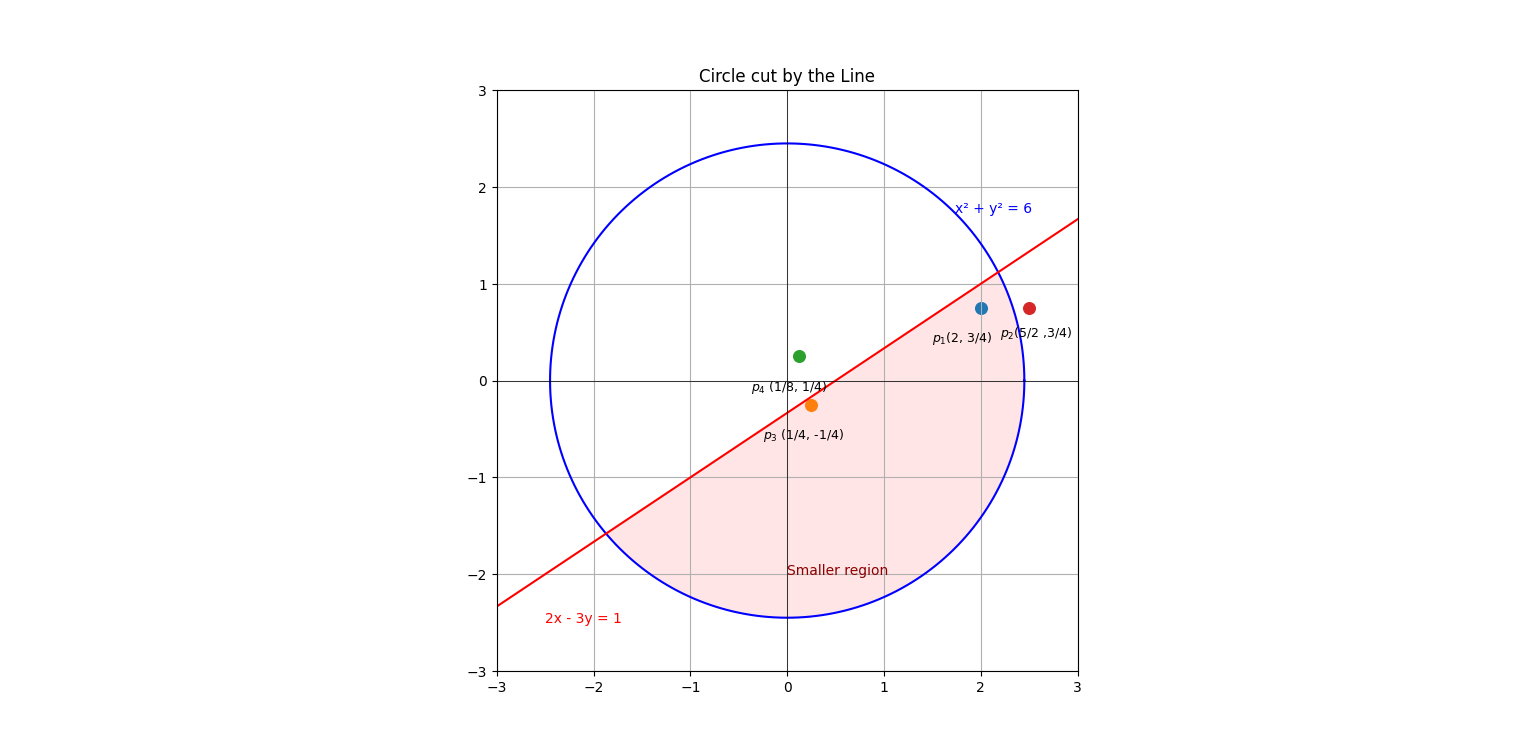
\includegraphics[width=\columnwidth]{figs/figure_py.png}
    \caption{Graph}
    \label{fig:fig}
 \end{figure}
\end{document}